\documentclass[10pt]{article}
\usepackage[polish]{babel}
\usepackage[utf8]{inputenc}
\usepackage[T1]{fontenc}
\usepackage{graphicx}
\usepackage[export]{adjustbox}
\graphicspath{ {./images/} }

\title{LIGA MATEMATYCZNA im. Zdzisława Matuskiego PÓŁFINAŁ 28 lutego 2020 SZKOŁA PODSTAWOWA \\
 klasy IV - VI }

\author{}
\date{}


\begin{document}
\maketitle
\section*{ZADANIE 1.}
Łączna długość pociągu i mostu jest równa 190 m . W pewnym momencie pociąg całkowicie wjechał na most i teraz długość części mostu bez pociągu jest równa 110 m . Oblicz długość mostu i długość pociągu.

\section*{ZADANIE 2.}
Kopciuszek miał 100 ziaren maku. Wszystkie włożył do pięciu miseczek w taki sposób, że w dwóch pierwszych jest łącznie 30 ziaren, w drugiej i trzeciej 33 ziarna, a w trzeciej i czwartej 41 ziaren. W piątej jest o 11 ziaren więcej niż w pierwszej. Do której miseczki Kopciuszek włożył najmniej ziaren maku?

\section*{ZADANIE 3.}
Wszystkie smoki i smoczyce mają po sześć łap. Każdy samiec ma cztery głowy, a każda samica trzy głowy. Pewna smocza rodzina kupiła na jesienne pluchy 51 czapek i 84 sztuki kaloszy. Każdy członek rodziny na każdą głowę założył jedną czapkę, a na każdą łapę jeden kalosz. Ile smoków i smoczyc liczy ta rodzina?

\section*{ZADANIE 4.}
Z cyfr 1, 2, 3, 4 układamy liczby dwucyfrowe o różnych cyfrach. Ile jest takich liczb? Ile wśród nich jest liczb pierwszych?

\section*{ZADANIE 5.}
Ania wycięła z brystolu jednakowe kartoniki. Każdy jest prostokątem o bokach o długości 16 cm i 7 cm . Z pięciu takich kartoników dziewczynka ułożyła figurę, jak na rysunku. Oblicz obwód tej figury.\\
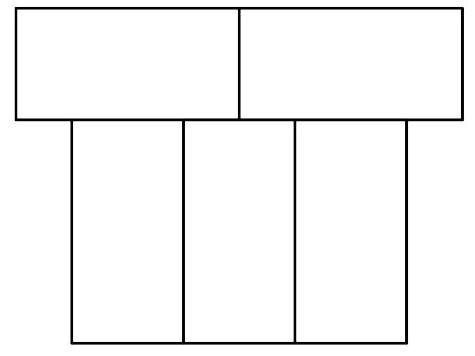
\includegraphics[max width=\textwidth, center]{2024_11_21_eba7c96c109b192ab548g-1}


\end{document}